\documentclass{article}
\usepackage[utf8]{inputenc}
\usepackage[backgroundcolor=yellow]{todonotes}
\usepackage{amsmath}
\usepackage{mathtools}
\usepackage{tikz}
\usetikzlibrary{matrix,shapes,arrows,positioning,chains, calc}
 
\title{Analysys of SQRL Authentication Protocol using proverif/spass/whatever}
\author{Dettoni, Claudio\\
	\texttt{cd611@cam.ac.uk}
	\and
	Perin, Lucas\\
	\texttt{lucas.perin@posgrad.ufsc.br}
}
\date{December 2016}

\begin{document}

\maketitle

\begin{abstract}
	In this paper we give a simple description of the SQRL authentication
	protocol and an analysys of a known vulnerability. We run an 
	experiment for formal verification of the protocul using ProVerif.
	Furthermore, we analyse a modified version of SQRL proposed to fix
	this vulnerability.
\end{abstract}

\section{Intoduction}
	Authentication protocols play an important role in modern internet
	usability. Most social network providers already have implemented
	some sort of authentication method to make it easy for users to connect
	to different services using the same account and credentials. Facebook \todo{Mention Oauth2a, Single Sign On}
	and google are fine examples of this. However, we know that the good and 
	old password is no longer reliable and has poor usability. \todo{Refs!!}
	Furthermore, most services on the web still use pass phrases for authentication,
	since this has been the main method used in previous decades. Hence,
	a common aproach to provide more security to personal accounts has 
	been the two-step verification, using and One Time Passwords (OTP) 
	provided by a trusted mobile app or token. This	method has gained some 
	space in authentication providers such as the
	ones previously mentioned. Therefore, we now have a mixed authentication process
	where the user can still use his passwords and be prompted for an
	OTP optionally.

	Numerous authentication protocols have been proposed in the past
	decade with the goal of replacing pass phrases with something that
	is actually secure and reliable for authentication providers. One
	good example is the Pico project \todo{ref}, with the main goal of
	completely removing passwords. Other examples of known protocols are ?, ? ?. \todo{enumerate and cite} 
	However, we have yet to see the adoption of one of these methods
	by a popular authentication provider to lead its use across the
	Internet. 

	In this paper, we analyse the SQRL protocol \todo{cite}. This protocol
	has drawed attention since its publication due to its simplicity. However,
	simple does not mean secure. In (?\todo{cite relay attack paper}) the authors
	describe how to use relay attacks to break through the SQRL authentication
	protocol. This attack can also be used with other authentication
	protocols that use images for authentication, such as Pico, ? and ?. \todo{enumerate}.
	Our goal is to use ProVerif, a tool for formal verification of cryptgraphic
	protocols, to demonstrate the SQRL protocol's vulnerability to relay attacks.
	Additionally, we use the same tool to verify a modification to this protocol 
	(proposed by the same author that describe the attack). \todo{conclude something}

\section{Secure Quick Reliable Login Protocol}

	The SQRL protocol, short for Secure Quick Reliable login, is an alternative method 
	for authentication replacing user names and passwords. It uses a QR code
	similar to other protocols, such as the Pico Project and TiQR. To log in
	the user should have a device that is capable of storing offline cryptographic
	keys and compute hash and cryptographic operations. In this work, we will consider that
	this is an application runing in an mobile device, namely the SQRL App. 
	Additionally, denote an existing authentication service provider as ASP. Now
	we can describe the main phases of the protocol as the \emph{Setup, Identity 
	Creation} and \emph{Authentication} phases.

	The \emph{Setup} phase is a standart cryptographic setup procedure where the
	SQRL App generates a random 256 bit master secret (MS). This secret is stored offline and 
	is never to be shared. The following phases will always be derivated of this
	secret, but never give it away. The \emph{Identity Creation} phase and the
	\emph{Authentication} phase are operations that should be syncronized with
	each ASP the user wants to authenticate to. In other words, the user will
	have to create an identity for each ASP and each ASP is responsible 
	for authenticating the user's credential upon log in.

	The \emph{Identity Creation} phase is performed when the user wishes to create an
	identity for a specific ASP. In this step he will create a Domain Secret (DS)
	derivated from the service's domain address and the MS, by using an HMAC function.
	This DS is used only for this specific ASP and no others. Furthermore, the
	MS should remain stored safely in case the user needs to create a new DS. In 
	this same phase, a public key (KU) and a private key (PK) are derived from the
	DS, where the KU is then forwarded to the ASP.


	The \emph{Authentication} phase should be the operation that users use the
	most. After the Setup and Identity Creation, the user should have a KU and
	a PK for each of his ASPs. To authenticate the user, the ASP generates a 
	nonce and displays it as a QR code for the user to scan. The user scans the
	nonce using the SQRL App and signs it with the PK. The signature is then
	sent to the ASP from the SQRL APP using a different communication channel,
	that is, a secure connection directly from the SQRL App and the ASP.
	Finally, the ASP verifies the signature received from the SQRL app and 
	approves or rejects the user's login attempt. See Figure \ref{fig:sqrlauth}

	\begin{figure}[ht]
	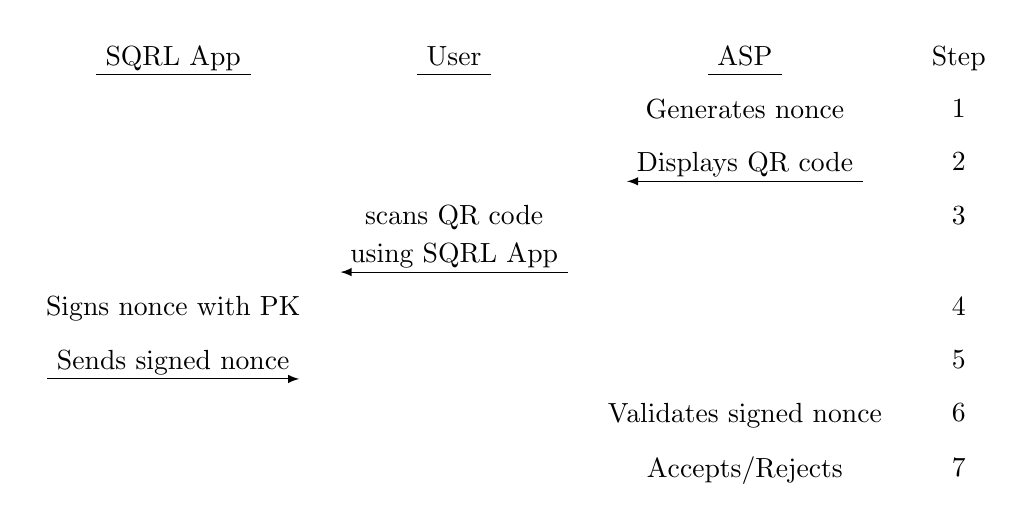
\begin{tikzpicture}
		\matrix (m)[matrix of nodes, column  sep=4mm,row  sep=2mm, 
					nodes={draw=none, anchor=center,text depth=0pt} ]
		{
		SQRL App & User & ASP & Step\\
		 & & Generates nonce & $1$ \\
		 & & Displays QR code & $2$ \\
		& scans QR code & & 3 \\[-2mm]
		& using SQRL App & & \\
		Signs nonce with PK & & & 4 \\
		Sends signed nonce & & & 5\\
		& & Validates signed nonce & 6\\
		& & Accepts/Rejects & 7\\
		};

		\draw (m-1-1.south east)--(m-1-1.south west);
		\draw (m-1-2.south east)--(m-1-2.south west);
		\draw (m-1-3.south east)--(m-1-3.south west);
		\draw[-latex] (m-3-3.south east)--(m-3-3.south west);
		\draw[-latex] (m-5-2.south east)--(m-5-2.south west);
		\draw[-latex] (m-7-1.south west)--(m-7-1.south east);
	\end{tikzpicture}
	\caption{SQRL Authentication Phase}
	\label{fig:sqrlauth}
\end{figure}


\subsection{Cryptographic Algorithm Remarks}
	The underlaying cryptographic algorithms used to generate random numbers, derivate
	key pairs from master secret and signature schemes are not detailed in this work.
	These are detailed and publicly availabe in the protocol's website (REF) and should not
	affect the attack we analyse here. 

\subsection{Security Remarks}
	The SQRL protocol, when used for website authentication, relies heavily on
	the \emph{Transport Layer Security} (TLS) cipher suite. The TLS ensures that
	the protocol phases should be secured with integrity, privacy and authenticity
	to prevent attacks such as the \emph{Man-in-the-middle} attack. A more extensive 
	analysis on the security of SQRL, can be foundin (REF) as well as in discussion 
	groups in the \emph{stack exchange} website.
	\todo[inline]{Update references}

\section{Similar Protocols}
\todo[inline]{OpenID, Pico, TiQR}

\section[Relay attack to visual code authentication schemes]{Relay attack to visual code \\
authentication schemes}
	The relay attack, as describe by the authors in (REF), is not a specific
	attack to the SQRL protocol, but rather to a family of protocol based on
	visual codes. Let us consider then a generic protocol that is compatible
	with the SQRL Authentication phase and other protocols in the same family.

	\begin{figure}[ht]
	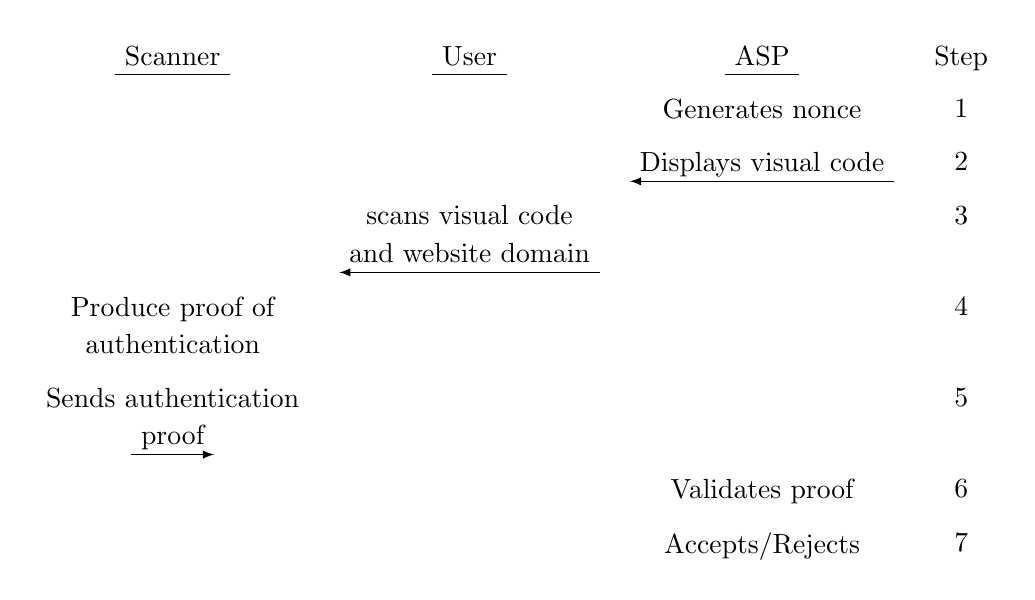
\begin{tikzpicture}
		\matrix (m)[matrix of nodes, column  sep=4mm,row  sep=2mm, 
					nodes={draw=none, anchor=center,text depth=0pt} ]
		{
		Scanner & User & ASP & Step\\
		 & & Generates nonce & $1$ \\
		 & & Displays visual code & $2$ \\
		& scans visual code & & 3 \\[-2mm]
		& and website domain & & \\
		Produce proof of& & & 4 \\[-2mm]
		authentication & & &\\
		Sends authentication & & & 5\\[-2mm]
		proof & & & \\
		& & Validates proof & 6\\
		& & Accepts/Rejects & 7\\
		};

		\draw (m-1-1.south east)--(m-1-1.south west);
		\draw (m-1-2.south east)--(m-1-2.south west);
		\draw (m-1-3.south east)--(m-1-3.south west);
		\draw[-latex] (m-3-3.south east)--(m-3-3.south west);
		\draw[-latex] (m-5-2.south east)--(m-5-2.south west);
		\draw[-latex] (m-9-1.south west)--(m-9-1.south east);
	\end{tikzpicture}
	\caption{General visual based authentication protocol}
	\label{fig:genauth}
\end{figure}


	\todo[inline]{Diagram with the protocol from relay attack paper}

	\todo[inline]{Continue}

	\todo[inline]{Diagram with the proposed fix to the protocols}

\section{Spass implementation}
\subsection{Overview of protocol verification with Spass}
	As shown in \todo[inline]{Towards an Automatic Analysis of Security Protocols in First-Order Logic}, 
	protocols can be interpreted using first-order logic. In this case, every message in the protocol
	is translated to logic assertions as well as the attacker capabilities, and then try to prove that the
	attacker cannot achieve some state that would lead to a failure.

	The parties knownledge are defined as logic predicates. For example, if party \emph{a} knows the message
	\emph{m}, then the predicate $Knows(a,m)$ is true. This same predicate could also be described, less 
	generically, as $Aknows(m)$ for example, but this does not make a difference in logical expressiveness.

	To represent the communication channel, the messages are translated to predicates meaning that they were
	sent and implications that manipulations to the knowledge of the parties. To emulate the parties behaviour,
	for example answering a message, the universal operator is used. The following example shows how a very simple
	protocol would be represented using first order logic. 

	$$ (i) A \rightarrow B:m  $$
	$$ (ii) B \rightarrow A:m $$

	In this simple procotol, A send a message to B that responds the same message. Using first-order logic the protocol
	would be written as the following:

	$$ sent(a,b,m) $$
	$$ \forall xa, xm \bullet  sent(xa,b,xm) \implies Knows(b, xm) \land  sent(b, xa, xm)$$

	The first assertion kick-starts the protocol, with $A$ sending the first message. The second assertion mimics $B$ 
	behaviour when receiving some message, which is replying the same message.

	To represent the attacker capabilities, one can say that the attacker can read anything in the channel,
	
	$$ \forall xa, xb, xm \bullet  sent(xa,xb,xm) \implies Knows(attacker, xm) $$

	or the attacker can send messages to anyone
	
	$$ \forall x, xm \bullet  Knows(attacker, xm) \implies sent(attacker, x, xm) $$

	To prove something regarding the protocol, we need to express this as a logical predicate and try to derive it from
	the described rules. For example, in the previously described protocol, does the attacker know $m$? This is true
	because:
		
	\begin{align*}
	\shortintertext{By definition}
	&sent(a,b,m)\\
	&\forall xa, xb xm \bullet  sent(xa,xb,xm) \implies Knows(attacker, xm)\\
	\shortintertext{Thus}
	&sent(a,b,m) \implies Knows(attacker, m)\\
	\shortintertext{By modus ponens}
	&Knows(attacker, m)\\
	\end{align*}

	Using this simple idea of logic predicates, more sophisticated protocols can be described. After fully writing them,
	one can try to prove more useful predicates, for example $Knows(attacker, key)$. Obviously, for complicated protocols
	there will be many logical assertions and it will be hard to make proofs manually. That is why Spass is useful as it
	is an automated first-order logic prover.
	

\section{Future Works}
	The experiments results in this work are not original, since the attack
	has been published and the authors are splicitly mentioned in our work.
	However, inspired by this, we can build a tool using spass/proverif to
	help protocol developers to detect the relay attack without too much
	effort.

\section{Final Remarks}
\todo[inline]{Some conclusion}


\end{document}
